\documentclass[11pt, a4paper, oneside]{Thesis} % Paper size, default font size and one-sided paper
\usepackage{wrapfig}
\usepackage{lscape}
\usepackage{rotating}
\usepackage{graphicx}
\usepackage{caption}
\usepackage{amsmath}

% custom packages
\usepackage{comment}
\usepackage{setspace}
\usepackage{subcaption}
\usepackage{float}
\usepackage{listings}
\lstset{
  language=sh,
  basicstyle=\ttfamily
}

% prints author names as small caps

%\usepackage{subcaption} %incompatible with subfig -- commented subfig package in Thesis.cls
\graphicspath{{Pictures/}} % Specifies the directory where pictures are stored
\usepackage[square, numbers]{natbib} % Use the natbib reference package - read up on this to edit the reference style; if you want text (e.g. Smith et al., 2012) for the in-text references (instead of numbers), remove 'numbers' v

\hypersetup{urlcolor=black, colorlinks=true} % Colors hyperlinks in blue - change to black if annoyingv`	
\title{\ttitle} % Defines the thesis title - don't touch this

% line spacing
\doublespacing

\begin{document}
\makeatletter
\renewcommand*{\NAT@nmfmt}[1]{\textsc{#1}}
\makeatother

% prints author names as small caps


\frontmatter % Use roman page numbering style (i, ii, iii, iv...) for the pre-content pages

\setstretch{1.6} % Line spacing of 1.6 (double line spacing)

% Define the page headers using the FancyHdr package and set up for one-sided printing
\fancyhead{} % Clears all page headers and footers
\rhead{\thepage} % Sets the right side header to show the page number
\lhead{} % Clears the left side page header

\pagestyle{fancy} % Finally, use the "fancy" page style to implement the FancyHdr headers

\newcommand{\HRule}{\rule{\linewidth}{0.5mm}} % New command to make the lines in the title page

% PDF meta-data
\hypersetup{pdftitle={\ttitle}}
\hypersetup{pdfsubject=\subjectname}
\hypersetup{pdfauthor=\authornames}
\hypersetup{pdfkeywords=\keywordnames}

%----------------------------------------------------------------------------------------
%	TITLE PAGE
%----------------------------------------------------------------------------------------

\begin{titlepage}
\begin{center}

\HRule \\[0.4cm] % Horizontal line
{\huge \bfseries \ttitle}\\[0.4cm] % Thesis title
\HRule \\[1.5cm] % Horizontal line
 
\large \textit{A thesis submitted in fulfilment of the requirements\\ for the degree of \degreename}\\[0.3cm] % University requirement text
\textit{by}\\[0.4cm]%

\href{http://home.iitk.ac.in/~saiwal}{\authornames}

\vfill
\graphicspath{ {./Figures/} }
\begin{figure}[hb]
  \centering
  
\includegraphics[width=0.4\linewidth]{Pictures/redlogo.jpg}
\end{figure}

\DEPTNAME\\ % Research group name and department name
\textsc{ \UNIVNAME}\\[1.5cm] % University name
\large \today\\[2cm] % Date


\end{center}

\end{titlepage}

%----------------------------------------------------------------------------------------
%	DECLARATION PAGE
%	Your institution may give you a different text to place here
%----------------------------------------------------------------------------------------

\Declaration{\addtocontents{toc}{\vspace{1em}} % Add a gap in the Contents, for aesthetics

It is certified that the work contained in this thesis entitled ''\ttitle'' by ''\authornames'' has been carried out under my supervision and that it has not been submitted elsewhere for a degree.
\\[2cm]

\begin{minipage}{0.4\textwidth}
	\begin{flushleft} \large
		\emph{\large \today}\\[2cm] % Date
	\end{flushleft}
\end{minipage}
\begin{minipage}{0.65\textwidth}
	{\begin{center} \large
		\supname
		\begin{center}
			{Professor\\ 
			\normalsize{\deptname\\
			\univname}}
		\end{center}
	\end{center}}
\end{minipage}
\vfill{}}

\clearpage % Start a new page

%----------------------------------------------------------------------------------------
%	ABSTRACT PAGE
%----------------------------------------------------------------------------------------

\addtotoc{Abstract} % Add the "Abstract" page entry to the Contents

\abstract{\addtocontents{toc}{\vspace{1em}} % Add a gap in the Contents, for aesthetics

UAVs have received considerable attention in the last decade, both in industry and academia. Potential applications are wide and varied, encompassing both military and domestic spaces. Search and rescue missions during disasters, environmental monitoring and surveillance, precision agriculture and farming are some of the domestic applications, while the scope of their usage in military space can be readily appreciated.

Communication is a critical component in realizing swarms of UAVs. There are two aspects of the communication architecture while considering UAV swarms. While there needs to be a reliable communication between the UAVs and a ground station, communication between individual UAVs is essential in enabling a distributed architecture for swarm applications. Wireless ad-hoc networks offer an appealing solution for inter UAV communication. While there have been works which used 802.11 based ad-hoc networks for the communication in multi UAV setups, these are short range links which are not suitable for the long range link between UAVs and the ground station. On the other hand, the commonly used 900 Mhz based radios for the communication between UAVs and the ground station in long range, are not well suited for inter UAV communication.

In this work, we present a novel communication architecture for UAV swarms, which combines both the long range and short range architectures. Moreover, our communication architecture is based on Robot Operating System(ROS), which ensures that any distributed application can be easily integrated into, and extended by the capabilities of ROS.
}

\clearpage % Start a new page

%----------------------------------------------------------------------------------------
%	ACKNOWLEDGEMENTS
%----------------------------------------------------------------------------------------

\setstretch{1.3} % Reset the line-spacing to 1.3 for body text (if it has changed)

\acknowledgements{\addtocontents{toc}{\vspace{1em}} % Add a gap in the Contents, for aesthetics

First and foremost, I would like to express my sincere gratitude and appreciation to my supervisor Dr. Ketan Rajawat. I am forever indebted to him for his expert guidance, continuous encouragement and steadfast belief in me, even when I myself had doubts in me. I feel extremely fortunate and am grateful to him for giving me an oppurtunity to work in this project, during which I had a fantastic learning experience.

I particularly offer my gratitude to Mohan and Lavish, who have been extremely supportive of me. The discussions we have had on diverse topics, throughout my stay at SPIN lab are invaluable. I would also like to thank Sanku and Anway with whom I have had a great pleasure of working. I also offer my thanks to all my peers in SPIN lab.

I fondly cherish my memories in IITK with my friends Suraj and Venkatesh, without whom these past two years would have much more difficult.

Last but not least, I express my profound gratitude to my parents, siblings and siblings-in-law, without whose unconditional love and unwavering support, this work would not have been possible.

}
\clearpage % Start a new page

%----------------------------------------------------------------------------------------
%	LIST OF CONTENTS/FIGURES/TABLES PAGES
%----------------------------------------------------------------------------------------

\pagestyle{fancy} % The page style headers have been "empty" all this time, now use the "fancy" headers as defined before to bring them back

\lhead{\emph{Contents}} % Set the left side page header to "Contents"
\tableofcontents % Write out the Table of Contents

\lhead{\emph{List of Figures}} % Set the left side page header to "List of Figures"
\listoffigures % Write out the List of Figures

\begin{comment}
\lhead{\emph{List of Tables}} % Set the left side page header to "List of Tables"
\listoftables % Write out the List of Tables

%----------------------------------------------------------------------------------------
%	ABBREVIATIONS
%----------------------------------------------------------------------------------------

\clearpage % Start a new page

\setstretch{1.5} % Set the line spacing to 1.5, this makes the following tables easier to read

\lhead{\emph{Abbreviations}} % Set the left side page header to "Abbreviations"
\listofsymbols{ll} % Include a list of Abbreviations (a table of two columns)
{
\textbf{FEA} & \textbf{F}inite \textbf{E}lement \textbf{A}nalysis \\
\textbf{FEM} & \textbf{F}inite \textbf{E}lement \textbf{M}ethod \\
\textbf{LVDT} & \textbf{L}inear \textbf{V}ariable \textbf{D}ifferential \textbf{T}ransformer \\
\textbf{RC} & \textbf{R}einforced \textbf{C}oncrete
%\textbf{Acronym} & \textbf{W}hat (it) \textbf{S}tands \textbf{F}or \\
}

%----------------------------------------------------------------------------------------
%	PHYSICAL CONSTANTS/OTHER DEFINITIONS
%----------------------------------------------------------------------------------------
%
%\clearpage % Start a new page
%
%\lhead{\emph{Physical Constants}} % Set the left side page header to "Physical Constants"
%
%\listofconstants{lrcl} % Include a list of Physical Constants (a four column table)
%{
%Speed of Light & $c$ & $=$ & $2.997\ 924\ 58\times10^{8}\ \mbox{ms}^{-\mbox{s}}$ (exact)\\
%% Constant Name & Symbol & = & Constant Value (with units) \\
%}

%----------------------------------------------------------------------------------------
%	SYMBOLS
%----------------------------------------------------------------------------------------

\clearpage % Start a new page

\lhead{\emph{Symbols}} % Set the left side page header to "Symbols"

\listofnomenclature{lll} % Include a list of Symbols (a two column table)
{
$D^{el}$ & elasticity tensor \\
$\sigma$ & stress tensor \\
$ \varepsilon $ & strain tensor \\
% Symbol & Name & Unit \\

}

\end{comment}

%----------------------------------------------------------------------------------------
%	DEDICATION
%----------------------------------------------------------------------------------------
%
\setstretch{1.3} % Return the line spacing back to 1.3
%
\pagestyle{empty} % Page style needs to be empty for this page
%
\dedicatory{I dedicate this work to my parents and teachers} % Dedication text
%
\addtocontents{toc}{\vspace{2em}} % Add a gap in the Contents, for aesthetics

%----------------------------------------------------------------------------------------
%	THESIS CONTENT - CHAPTERS
%----------------------------------------------------------------------------------------
% double spacing for the normal body
\doublespacing

\mainmatter % Begin numeric (1,2,3...) page numbering

\pagestyle{fancy} % Return the page headers back to the "fancy" style

% Include the chapters of the thesis as separate files from the Chapters folder
% Uncomment the lines as you write the chapters

% Chapter Template
% \doublespacing

\chapter{Introduction} % Main chapter title

\label{Chapter1} % Change X to a consecutive number; for referencing this chapter elsewhere, use \ref{ChapterX}

\lhead{Chapter I. \emph{Introduction}} % Change X to a consecutive number; this is for the header on each page - perhaps a shortened title

%----------------------------------------------------------------------------------------
%	SECTION 1
%----------------------------------------------------------------------------------------

\section{Rise of Unmanned Aerial Vehicles}
Unmanned aerial vehicles or UAVs have become ubiquitous in the past decade, both in research and industry. A myriad of applications involving UAVs in diverse fields has made them quite popular. Potential domestic  applications include Environmental monitoring and surveillance \cite{envmon}, traffic management \cite{trasur}, remote sensing \cite{remsen}, precision agriculture and farming \cite{preagr}, disaster management \cite{disman}, to name a few. The use of UAVs for defence purposes is only poised to grow in the next decade. It is not hard to see the appeal of UAVs in the defence sector with applications ranging from simple surveillance and reconnaissance missions to offensives like \textit{search and destroy} missions and targeted hits.

Much of the rise of this interest in UAVs can be attributed to associated advances in robotics, largely driven by the progress in robust and cheap sensors and communication technology. The emergence of scalable and extensible software architectures like the Robot Operating System(ROS), which enables easy integration of various subsystems further pushed the progress in these domains.

While early applications of UAVs were single UAV based, the focus is now shifting towards applications involving multiple UAVs, cooperatively completing tasks. There are several advantages of multi-UAV systems over single UAV systems. In certain applications like search and rescue missions, for instance, the use of multiple UAVs for surveying an area can significantly reduce the time taken to complete the task \cite{coosea}. As given by \cite{fanets}, other advantages of multi-UAV systems over single UAV systems include cost, scalability, survivability and speed.

Though UAV swarms have promising capabilities, they have quite a few challenges to overcome. Communication is one of the main hindrances to realize robust swarms of UAVs.

\section{The Challenge of Communications in UAV swarms}
While there is much literature regarding communication in UAV systems, \cite{fanets} and \cite{lavgupta} are two good survey articles regarding the current trends and issues in communication in UAV swarms. Besides pointing out the shifting interest towards multi UAV systems, due to their advantages over single UAV systems, they also identify the challenges in these systems, communication among the UAVs being the most notable one. 

Since the first applications were single UAV based, communication architecture in these systems was simple and straightforward. Often, there only needed to be a communication link between the UAV and the ground station. In some cases where the UAV has to cover a larger area, there could be multiple ground stations, and the UAV would have to communicate with the ground station near it. Even then, the overall architecture was pretty basic. As we noted earlier, there is a rapidly growing interest in realizing swarms of cooperative and collaborative UAVs, accomplishing complex tasks. Robust and reliable communication among the UAVs is an essential and critical component in enabling cooperative and collaborative behaviour in these UAV swarms.

While there is some interest in infrastructure based communication in UAVs, like using cellular infrastructure for UAVs \cite{celsur}, much of the research community considers enabling UAV communications in infrastructure less environments, more significant. These so called adhoc networks are important, for instance in disaster management scenarios where the existing infrastructure is damaged, or in military applications where there is no pre-existing infrastructure. The authors in \cite{lavgupta} try to identify several possible communication architectures for multi UAV networks.

\begin{figure}
	\centering
	\begin{subfigure}[b]{0.3\textwidth}
		\centering
		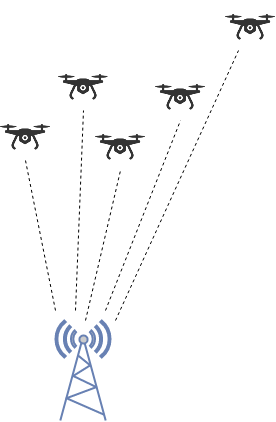
\includegraphics[scale=0.45]{Pictures/star.png}
		\caption{Star Configuration}
		\label{fig: starconf}
	\end{subfigure}
	\begin{subfigure}[b]{0.3\textwidth}
		\centering
		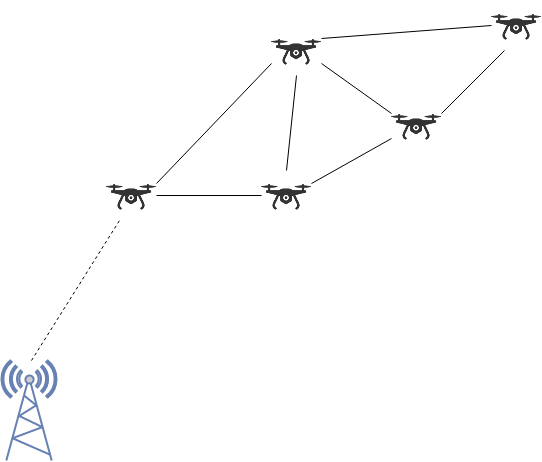
\includegraphics[scale=0.45]{Pictures/mesh.png}
		\caption{Mesh Configuration}
		\label{fig: meshconf}
	\end{subfigure}
	\caption{Possible network configurations for communications in UAVs}
	\label{fig: netconf}
\end{figure}

Figure \ref{fig: starconf} shows the star topology, where all the UAVs are connected to the ground station. In this configuration, the necessary communication among UAVs also needs to be routed through the ground station. Figure \ref{fig: meshconf} shows the mesh topology, where the UAVs communicate among themselves using an adhoc network, they themselves form. Typically, the ground station is also a part of the adhoc network. In the star configuration, since all the data has to be routed through the ground station, there would be higher latency and congestion in the network.

On top of that, if the UAVs are considerably far from the ground station, the network in star configuration may not provide reasonably high bandwidth for the communication among the UAVs. Moreover, if any of the UAVs loses its link to the ground, it cannot be accessible by any other UAVs, even if they are close. It is clear to see that the mesh configuration has a considerable advantage over the star configuration. Indeed, there is a consensus in the literature that realizing adhoc networks is the best solution for communication in multi UAV systems. There is a growing intereset in FANETs, the Flying Adhoc Networks. There is much literature in the filed and \cite{fanets} introduces and outlines the current and future trends in FANETs.

\begin{comment}
\section{FANETs, Flying Adhoc Networks}
While there were early attempts at different names for adhoc networks in UAVs like AUGNET \cite{augnet} and UAVNET \cite{uavnet}, the name FANET seems to be favoured. 

FANETs come under more general adhoc networks called MANETs(Mobile Adhoc Networks) and VANETs(Vehicular Adhoc Networks). MANET is the most general of the both and the oldest. There have been MANET protocols and standards defined to an extent.
\end{comment}

\section{Motivation and the Current Work}
With the advent of Internet of Things(IOT), there are now several communication standards which enable mesh networks like Bluetooth mesh networks \cite{blemesh}, Thread \cite{thread, thread2} and Zwave \cite{zwave}, where the last two protocols are based on the IEEE standard 802.15 \cite{meshsurvey}. Despite these, mesh networks which are based on the wifi, as standardized in IEEE 802.11s, better suit the needs of UAVs because of their high data rate and range.

While there are previous works which have used wifi based adhoc networks in UAVs like AUGNET \cite{augnet} and UAVNET \cite{uavnet}, they have several issues, not least of which is the range of the networks. Though the mesh networks enable reliable communication among the UAVs at an acceptable range, the link between the UAVs and the ground station is much more vulnerable. While the distance between the neighbouring UAVs can be kept relatively small, one cannot restrict the distance between the ground station and a UAV. A typical scenario would be that of a group of UAVs flying as a swarm far from the ground station. Even though the UAVs are in range and allow communication among themselves via the wifi mesh, the ground station at a larger distance can no longer be a part of the mesh. This is certainly a limiting factor in mesh networks for UAVs. This is one of the motivations for this work, in which we address this issue by using two different radio modules, a long range and a short range one(the wifi mesh). We propose a new architecture which blends short range and long range aspects of the communication. Note that the long range radios typically provide low bandwidth and are not suited for robust inter communication among the UAVs, demanded by many emerging distributed applications. This is not a concern in the case of the link between the UAVs and the ground station as long as, much data is not needed at the ground station, which is the case in autonomous applications, where much of the decision making happeds on board the UAV and ground station is merely used for monitoring.

Another aspect of motivation for this work is its integration with the Robot Operating System or ROS. ROS is a widely accepted software platform for research in robotics, which became popular as \textit{Linux for Robotics.} ROS, with its distributed and modular architecture, active development, collabarative environment and vibrant community has seen widespread adoption by individuals and organizations, across the board in robotics research. Thus the goal was to integrate our communication architecture into ROS, enabling development of distributed applications among UAVs without the need to worry about the underlying communication architecture.

\section{Organizaiton of the thesis}
We have introduced and motivated the problem of communication in UAV swarms in chapter \ref{Chapter1}. In chapter \ref{Chapter2}, we shall look at the development of the mesh architecutre. We shall look at the long range communication architecture in chapter \ref{Chapter3}. We shall look at some future work and  finally conclude this thesis with chapter \ref{Chapter4}.
% Chapter Template

\chapter{The Mesh Architecture} % Main chapter title

\label{Chapter2} % Change X to a consecutive number; for referencing this chapter elsewhere, use \ref{ChapterX}

\lhead{Chapter 2. \emph{The Mesh}} % Change X to a consecutive number; this is for the header on each page - perhaps a shortened title

In this chapter, we will look at the short range communication architecture for inter communication among the UAVs which entails realizing a wifi mesh network based on the IEEE standard 802.11s. We shall also look at how it is integrated into ROS.

%----------------------------------------------------------------------------------------
%	SECTION 1
%----------------------------------------------------------------------------------------

\section{IEEE 802.11s}
The IEEE WLAN 802.11 standard is quite a popular solution for high bandwidth networking services at reasonable distances. But, it is based on a centrailized architecture, where every networking node is a \textit{Station}, STA. In the simplest architecture, one of the STAs acts as an \textit{Access point}, AP, a centralized node which provides integration services to other STAs. It is a single hop architecture where \textit{STAs} directly communicate with \textit{APs}, and all the communication between \textit{STAs} is routed through the \textit{AP} to which they are connected. Essentially, it is a network in star configuration, at MAC layer.

With growing demand for more diverse wireless infrastructure and multihop networks, 802.11s \cite{802.11s} emerged as an ammendment to the original standard to accommodate mesh networking architecture. The 802.11s standard extends the 802.11 MAC layer, allowing a MAC based multihop architecture.

\begin{figure}
	\centering
	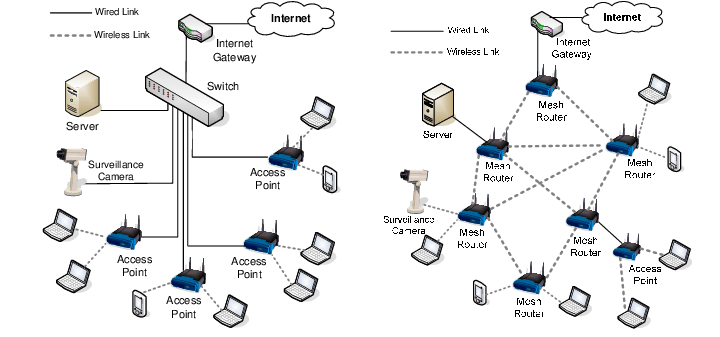
\includegraphics[scale=0.6]{Pictures/80211s.png}
	\caption{A comparison of 802.11 wlan and 802.11s mesh networks}
	\label{fig: 80211s}
	\captionsetup{font={footnotesize,bf,it}}
	\caption*{source: Portmann, Marius. (2006). Wireless Mesh Networks for Public Safety and Disaster Recovery Applications. 10.1201/9781420013542.ch16. }
\end{figure}

\subsection{Routing in 802.11s}
Though there are a lot of routing protocols proposed in wireless mesh networks, the field is still active in research. What routing protocol to use closely depends on the application, and choice of the routing protocol may significantly impact the performance of the system. Different routing protocols can be mainly categorized into two types.
\begin{itemize}
	\item{\textit{Proactive Routing Protocols:} Proactive routing protocols are those protocols where the nodes keep track of the routes of all the accessible nodes. This is done by some information about the topology of the network, }
\end{itemize}









 
% Chapter Template

\chapter{Long Range Communication Architecture} % Main chapter title

\label{Chapter3} % Change X to a consecutive number; for referencing this chapter elsewhere, use \ref{ChapterX}

\lhead{Chapter 3. \emph{Long Range Communication}} % Change X to a consecutive number; this is for the header on each page - perhaps a shortened title

In this chapter, we shall look at the long range communication architecture, menat for communication between ground station and the UAVs, and how it is integrated with the mesh network and ROS.

\section{Hardware}
Among the existing solutions for long range communication, radios based on 900Mhz spectrum seem popular. Compared to 2.4Ghz radios, there are a few reasons for this. First, the path loss for 2.4Ghz radios is higher than that of 900Mhz radios, reducing the received signal strength significantly over long distances. With the use of high gain directional antennas, the gap in the received signal strength between the radios of two spectra, can be eliminated, or even reversed. While this makes the 2.4Ghz radios favorable than 900Mhz radios in static point-to-point links, 900Mhz radios still have a much longer range than 2.4Ghz radios. Second, the 2.4Ghz spectrum is more vulnerable to the issues of penetration and blockages in the face of obstacles, while 900Mhz is more robust to them.

Note that much of 2.4Ghz hardware consists of wifi based solutions, based on the 802.11 hardware, and 802.11 was designed to be indoor, with short range, but high bandwidth. Consequently, hardware based on 802.11 is inefficient for use over long distances. While there are implementations of custom protocol stacks, instead of 802.11, on 2.4Ghz spectrum, these are almost always propietary and consequently, the modules are quite expensive. Considering all things, 900Mhz radios are still offer quite a promising solution for communication over long distances. One downside is that the 900Mhz radios typically offer lower bandwidth on the order of a few 100 Kbps, compared to 2.4Ghz solutions. Nonetheless, this should not be a problem as long as not too much data is demanded at the ground station, which is true in most applications.

\subsection{RFD900X}
RFD900X is third in line of popular 900Mhz radios by the company, RFDesign, the first two being RFD900 and RFD900+. The radio operates on frequency range 902-928 Mhz. It allows selectable transmit power upto 30dBm, in steps of 1dBm. It supports multiple air data rates from 4Kbps to 500Kbps. It has a UART interface supporting multiple baud rates from 9600 to 1000000. It has an advertised range of more than 50Kms in line of sight conditions, depending on antennas. The radios support a set of AT commands for configuring different parameters. There is decent documentation regarding the radios that can be found at \url{http://files.rfdesign.com.au/docs/}.

\begin{figure}[h]
	\centering
	\begin{subfigure}{0.5\textwidth}
		\centering
		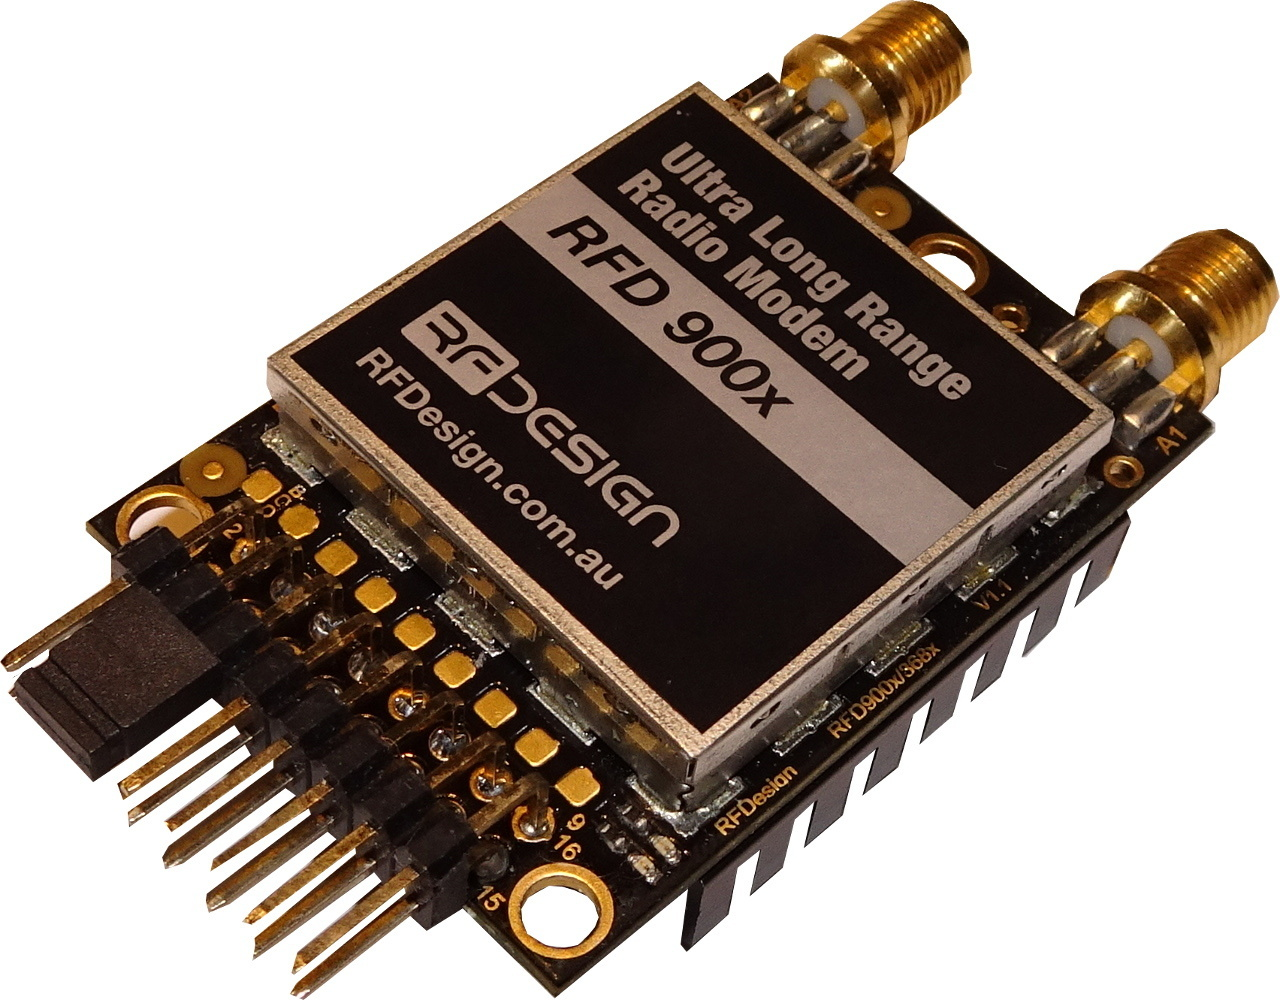
\includegraphics[scale=0.1]{Pictures/rfd1.jpg}
	\end{subfigure}%
	\begin{subfigure}{0.5\textwidth}
		\centering
		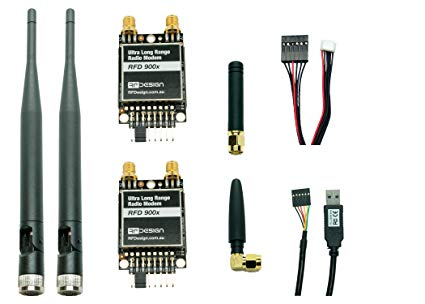
\includegraphics[scale=0.5]{Pictures/rfd2.jpg}
	\end{subfigure}
	\caption{RFD900x along with antennas and FTDI cables}
	\label{fig: rfd900x}
\end{figure}

The radios come with a default peer to peer firmware, which means that the radios can only be used in pairs. There are two other firmwares that can be flashed on radios, synchronous mesh and asynchronous mesh, which are point to multipoint firmwares. These firmwares can be flashed by a gui program called 'Modem Tools' that can downloaded from \url{http://files.rfdesign.com.au/}.

\subsubsection{Peer to Peer Firmware}
As mentioned, the radios come flashed with the peer to peer firmware by default. We may need to configure the radios with some parameters via the AT commands. For instance, the parameters NETID, SERIAL\_SPEED, AIR\_SPEED should be same on both the modems, among other things. Radios with same NETID can talk to each other. Essentially, any raw bytes input to the serial UART interface at one radio can be received at the serial interface of the other radio. Different pairs of radios with different NETIDs can only send and receive data to and from the radio with the same NETID. Even though you can have multiple pairs of radios wiht different NETIDs, as the total number of radios increase, interference also increases, increasing the errors in transmitted bytes.

\begin{figure}[h]
	\centering
	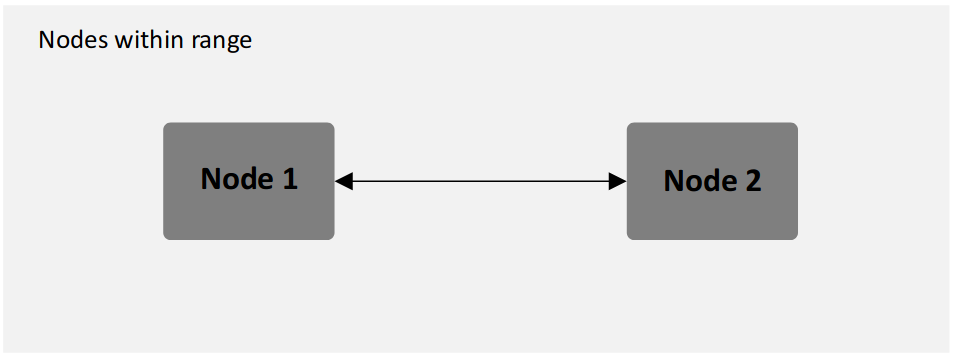
\includegraphics[scale=0.4]{Pictures/peer.png}
	\caption{modems in peer to peer configuration}
	\label{fig: rfdpeer}
	\captionsetup{font={footnotesize,bf,it}}
	\caption*{source: http://files.rfdesign.com.au/Files/documents/RFD900x\%20DataSheet\%20V1.1.pdf}
\end{figure}

\subsubsection{Synchronous Mesh Firmware}
While the peer to peer firmware allows communication only between a pair of radios, the asynchronous firmware is a point to multipoint firmware. Apart from the NETID parameter, there is a NODEID parameter, NODEDESTINATION parameter, NETCOUNT parameter among others, that can be set by the AT commands. Unlike the peer to peer firmware, more than two radios can have the same NETID. While using the synchronous firmware, one of the radios needs to be as a base node. This can be done by setting the NETID parameter to 0 and NODEID parameter to 1 on the base radio. We should also specify the number of radios with the parameter NETCOUNT.

In this configuration, the base radio assigns time slots to each of the other radios to communicate. Essentially, each radio transmits data only during its assigned time slot. So, even if other radios are not transmitting data, a radio waits for its time slot to transmit its data. This is inefficient when either not many radios are transmitting or they are not transmitting too often.

\begin{figure}[h]
	\centering
	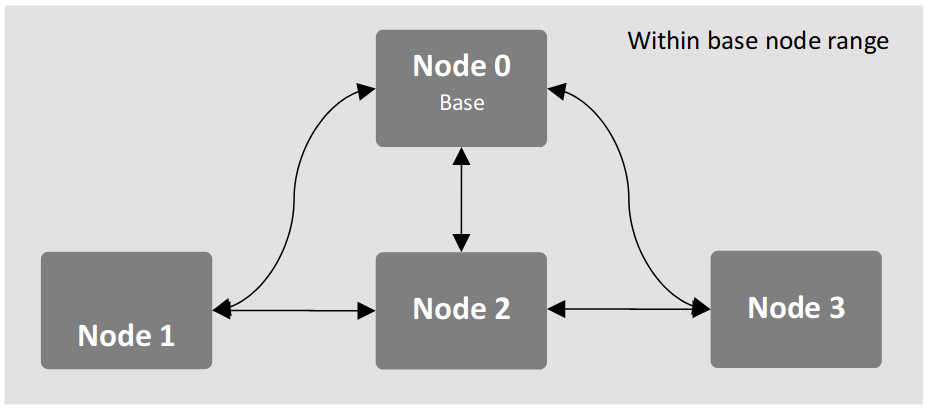
\includegraphics[scale=0.4]{Pictures/sync.png}
	\caption{modems in synchronous mesh configuration}
	\label{fig: rfdsync}
	\captionsetup{font={footnotesize,bf,it}}
	\caption*{source: http://files.rfdesign.com.au/Files/documents/RFD900x\%20DataSheet\%20V1.1.pdf}
\end{figure}





% Chapter Template

\chapter{Conclusion} % Main chapter title

\label{Chapter4} % Change X to a consecutive number; for referencing this chapter elsewhere, use \ref{ChapterX}

\lhead{Chapter 4. \emph{Conclusion}} % Change X to a consecutive number; this is for the header on each page - perhaps a shortened title

We proposed and implemented a novel communication architecture for emerging applications in UAVs, using off the shelf hardware. The architecture blends both short range and long range communication systems. For short range communication, we realize a wifi mesh network among the UAVs, using commercially available wifi routers. We achieve this by using an embedded linux operating system for routers called, OpenWrt. This mesh network enables robust and reliable communication among the UAVs for distributed applications like swarm formation and control, localization, cooperative search, to name a few.

We integrate this architecture with a long range communication system for communication with the ground station. We use popular 900Mhz radios called RFD900x as our long range modules. We propose two architectures, \textit{Static Leader} and \textit{Dynamic Leader}, where the second one is an extension of the first one. In \textit{Static Leader}, we designate one of the UAVs as \textit{leader} which transmits data to the ground station. In \textit{Dynamic Leader}, the \textit{leader} is not set apriori, but chosen dynamically by the UAVs themselves.

The integration of the long range communication sytem with the short range mesh network enhances the effective range of the operations that can be conducted with the  UAVs. Furthermore, our architecture is integrated into ROS. This makes our architecture quite flexible, in the sense that it enables anyone to develop their multiple UAV applications in ROS without worrying about the underlying communication architecture. Both the \textit{Static Leader} and \textit{Dynamic Leader} architectures are implemented in two open source ROS packages \textit{serialros} and \textit{swarmBaba}. The source code and implementation can be found at \url{https://github.com/saiadityachundi/serialros} and \url{https://github.com/saiadityachundi/swarmBaba}.

\section{Future Work}
While we have designed and implemented this architecture and tested it indoors, we haven't done extensive outdoor testing. Hence, one of the directions for future work is to do extensive outdoor testing and measure the range over which this architecture reliably works.

Also, the long range radio modules we have used were RFD900x which were serial radios. There are some alternatives to these radios which offer IP based solutions in 900Mhz spectrum. While it would be much easier to integrate an IP based radio into the ROS framework, it is still worthy exercise. There are other proprietary radio solutions in 2.4Ghz spectrum, apart from the normal 802.11 standard, which claim to offer much longer ranges than traditional wifi. Working with these different radios and implementing a similar architecture is worth pursuing.
%% Chapter Template

\chapter{Preliminaries} % Main chapter title

\label{Chapter5} % Change X to a consecutive number; for referencing this chapter elsewhere, use \ref{ChapterX}

\lhead{Chapter 5. \emph{Preliminaries}} % Change X to a consecutive number; this is for the header on each page - perhaps a shortened title

In this chapter, we shall briefly look at all the components present in a general autonomous UAV.

\begin{figure}[h]
	\centering
	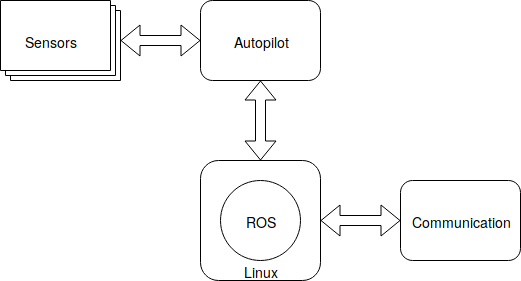
\includegraphics[scale=0.8]{Pictures/uav.png}
	\caption{Components in a general autonomous UAV}
	\label{fig: uav}
	\captionsetup{font={footnotesize,bf,it}}
\end{figure}

Figure \ref{fig: uav} shows several subsytems in an an autonomous UAV we consider. It consists of an autopilot which is handles low level control of the UAV dynamics. The autopilot is responsible for attitude stabilization, for instance, in quadrotors. It directly connects with 
  
%\input{Chapters/Chapter6} 
%\input{Chapters/Chapter7}

%----------------------------------------------------------------------------------------
%	THESIS CONTENT - APPENDICES
%----------------------------------------------------------------------------------------
\begin{comment}
\addtocontents{toc}{\vspace{2em}} % Add a gap in the Contents, for aesthetics

\appendix % Cue to tell LaTeX that the following 'chapters' are Appendices

% Include the appendices of the thesis as separate files from the Appendices folder
% Uncomment the lines as you write the Appendices

\input{Appendices/AppendixA}
%\input{Appendices/AppendixB}
%\input{Appendices/AppendixC}

\addtocontents{toc}{\vspace{2em}} % Add a gap in the Contents, for aesthetics
\end{comment}
\backmatter

%----------------------------------------------------------------------------------------
%	BIBLIOGRAPHY
%----------------------------------------------------------------------------------------
% single spacing for bibliography
\singlespacing

\nocite{*}
\label{Bibliography}

\lhead{\emph{Bibliography}} % Change the page header to say "Bibliography"

\bibliographystyle{apalike} % Use the "custom" BibTeX style for formatting the Bibliography

\bibliography{Bibliography} % The references (bibliography) information are stored in the file named "Bibliography.bib"

\end{document}